%%%%%%%%%%%%%%%%%%%%%%%%%%%%%%%%
% Section 3 (method+theory): definition -> early exploration (lower env)
%   -> late annealing (upper env) -> branch opening + Pass@N
% All formal proofs are deferred to Appendix~\ref{app:proofs}.
%%%%%%%%%%%%%%%%%%%%%%%%%%%%%%%%

\section{Random Soft Prompts and Why They Work}\label{sec:why_rsp_works}

This section defines Random Soft Prompts (RSPs) and explains their behavior in two parts. A single RSP draw is fixed within one rollout and selects one branch different from baseline. Its influence is meaningfully large at early tokens (\S\ref{sec:improve}) and automatically converges to zero as decoding proceeds (\S\ref{sec:converge}). Because each rollout draws a fresh RSP, the across-rollout differences accumulate into Pass@$N$ improvements at an exponential rate (\S\ref{sec:multipath}). The body keeps theorem statements and intuition; all formal proofs are deferred to Appendix~\ref{app:proofs}.

% ================================================================
\subsection{Random Soft Prompt}\label{sec:rsp_definition}
% ================================================================

The construction is simple: borrow the entrywise mean and scale of the pretrained token embedding table to draw a continuous vector of the same shape, and concatenate it before, inside, or after the prompt.

Formally, let $\mathbf{W}_E \in \mathbb{R}^{V\times d}$ denote the token embedding matrix ($V$ is the vocabulary size, $d$ the hidden dimension), and write its entrywise mean and standard deviation as $\mu_E := \tfrac{1}{Vd}\sum_{i,k}[\mathbf{W}_E]_{i,k}$ and $\sigma_E := \mathrm{std}(\mathbf{W}_E)$. An RSP of length $L$ is a sequence of continuous vectors $\mathbf{H} = [h_1,\dots,h_L]\in\mathbb{R}^{L\times d}$ drawn independently from
\begin{equation}\label{eq:rsp_def}
h_j \;\sim\; \mathcal{N}(\mu_E\mathbf{1}_d,\;\sigma_E^2\mathbf{I}_d), \quad j=1,\dots,L.
\end{equation}
The centered form $\bar h_j := h_j - \mu_E\mathbf{1}_d \sim \mathcal{N}(0,\sigma_E^2\mathbf{I}_d)$ is a zero-mean isotropic Gaussian. The injection position into the input embedding sequence $\mathbf{X}$ is one of three: prefix $[\mathbf{H};\mathbf{X}]$, infix (insert $\mathbf{H}$ inside $\mathbf{X}$), or suffix $[\mathbf{X};\mathbf{H}]$ \citep{kang2025model, xu2025softcot, ye2025thinking, zhang2025memgen}. For repeated-sampling protocols, the prompt draws and decoding randomness across compared trials are assumed independent.

The role of randomness is not to imitate the embedding distribution. It is to ensure that the same prompt produces \emph{independent} perturbations across rollouts---and exploration is precisely what requires this independence.

% ================================================================
\subsection{Early exploration: a lower envelope}\label{sec:improve}
% ================================================================

RSP does not add to the hidden state directly; it enters only through attention weights. Hence the entire instantaneous influence of RSP at one layer collects into a single scalar---the attention mass assigned to RSP tokens. Consider self-attention layer $\ell$ with $n$ real tokens and $L$ RSP tokens, attention weights $\alpha_{ij}^{(\ell)}$, and value vectors $\mathbf{v}_j^{(\ell)},\mathbf{v}_{r_j}^{(\ell)}$ on the real and RSP sides. Define $w_{r,i}^{(\ell)} := \sum_{j'=1}^L \alpha_{i,n+j'}^{(\ell)}$. The attention output decomposes exactly as
\begin{equation}\label{eq:decomp}
\mathbf{x}_i^{(\ell+1)}
= (1-w_{r,i}^{(\ell)})\,\tilde{\mathbf{x}}_i^{(\ell+1)} + \boldsymbol{\eta}_i^{(\ell)},
\quad
\tilde{\mathbf{x}}_i^{(\ell+1)} := \sum_{j=1}^n \tfrac{\alpha_{ij}^{(\ell)}}{1-w_{r,i}^{(\ell)}}\mathbf{v}_j^{(\ell)},
\quad
\boldsymbol{\eta}_i^{(\ell)} := \sum_{j'=1}^L \alpha_{i,n+j'}^{(\ell)}\mathbf{v}_{r_{j'}}^{(\ell)}.
\end{equation}
This identity uses only softmax normalization (derivation: Appendix~\ref{app:proofs}). Since $\|\boldsymbol{\eta}_i^{(\ell)}\| \le w_{r,i}^{(\ell)} \max_{j'}\|\mathbf{v}_{r_{j'}}^{(\ell)}\|$, the same scalar $w_{r,i}^{(\ell)} \in [0,1]$ controls both the attenuation ratio $1-w_{r,i}^{(\ell)}$ on the real-token signal and the upper bound on the random contribution's magnitude. The behavior of RSP reduces to tracking one value rather than a multidimensional perturbation.

The key question is whether this value is \emph{meaningfully nonzero} at early decoding. The following lower-envelope statement provides this guarantee. Let $\mathbf{q}_i^{(\ell)}$ be the query and $\mathbf{k}_j^{(\ell)}, \mathbf{k}_{r_{j'}}^{(\ell)}$ the real and RSP keys at layer $\ell$.

\begin{proposition}[Lower envelope for early exploration]\label{prop:lower_env}
Define the reverse logit gap $\Delta_i'^{(\ell)} := \max_{j\in[n]}(\mathbf{q}_i^{(\ell)})^\top\mathbf{k}_j^{(\ell)} - \min_{j'\in[L]}(\mathbf{q}_i^{(\ell)})^\top\mathbf{k}_{r_{j'}}^{(\ell)}$. Then in scaled dot-product attention, $w_{r,i}^{(\ell)} \ge L/(L + n\,\exp(\Delta_i'^{(\ell)}/\sqrt d))$.
\end{proposition}

The proof is in Appendix~\ref{app:proofs} (symmetric to Theorem~\ref{thm:decay} below). The bound equals 1 at $n=0$ and stays close to 1 while $n$ is small, provided $\Delta_i'^{(\ell)}$ is not excessively large. Hence \emph{when the reverse gap does not blow up}, early decoding inherits a strictly positive lower bound on RSP influence---a single very poor RSP key score, however, can inflate $\Delta_i'^{(\ell)}$ and weaken the bound.

% ================================================================
\subsection{Late convergence: an upper envelope and annealing}\label{sec:converge}
% ================================================================

The symmetric question is whether the same scalar \emph{converges to zero} at late decoding. Define the forward logit gap $\Delta_i^{(\ell)} := \min_{j\in[n]}(\mathbf{q}_i^{(\ell)})^\top\mathbf{k}_j^{(\ell)} - \max_{j'\in[L]}(\mathbf{q}_i^{(\ell)})^\top\mathbf{k}_{r_{j'}}^{(\ell)}$ ($\Delta_i^{(\ell)} \le \Delta_i'^{(\ell)}$).

\begin{theorem}[Upper envelope under annealing]\label{thm:decay}
In scaled dot-product attention, $w_{r,i}^{(\ell)} \le L/(L + n\,\exp(\Delta_i^{(\ell)}/\sqrt d))$. The right-hand side is strictly decreasing in $n$ at fixed $L$ and $\Delta_i^{(\ell)}$, and converges to zero as $n\to\infty$ in the fixed-gap regime.
\end{theorem}

The proof is in Appendix~\ref{app:proofs}. Combined with Proposition~\ref{prop:lower_env}, we obtain a two-sided sandwich:
\begin{equation}\label{eq:sandwich}
\frac{L}{L+n\,\exp(\Delta_i'^{(\ell)}/\sqrt d)} \;\le\; w_{r,i}^{(\ell)} \;\le\; \frac{L}{L+n\,\exp(\Delta_i^{(\ell)}/\sqrt d)}.
\end{equation}
Both envelopes equal 1 at $n=0$ and tend to 0 as $n\to\infty$, but \emph{at different rates} ($\Delta_i^{(\ell)}\le\Delta_i'^{(\ell)}$). Early on, both envelopes hover near 1; late on, both vanish. The theorem does not assert step-by-step monotonic decay of the realized mass---queries, keys, and hidden states co-evolve so both gaps shift over time. What it does guarantee is that the \emph{fixed-gap envelope narrows under cache growth alone}.

This means RSP behaves at each attention site as a local perturbation that briefly acts and then weakens. Defining the disturbance energy $V_{\eta,i}^{(\ell)} := \mathbb{E}\|\boldsymbol{\eta}_i^{(\ell)}\|^2$, a finite second moment $M_v^{(\ell)} := \max_{j'}\mathbb{E}\|\mathbf{v}_{r_{j'}}^{(\ell)}\|^2$ yields $V_{\eta,i}^{(\ell)} \le M_v^{(\ell)}(w_{r,i}^{(\ell)})^2$ (Appendix~\ref{app:rsp_noise}), and combining with Theorem~\ref{thm:decay} gives $V_{\eta,i}^{(\ell)} = O(1/n^2)$ in the fixed-gap regime. This is an upper bound at \emph{a single attention site}; it does \emph{not} claim that the full hidden-state trajectory $\|h_t^{\mathrm{RSP}} - h_t^{\mathrm{base}}\|$ decreases or that the transformer minimizes a global energy.

\begin{figure}[ht]
  \centering
  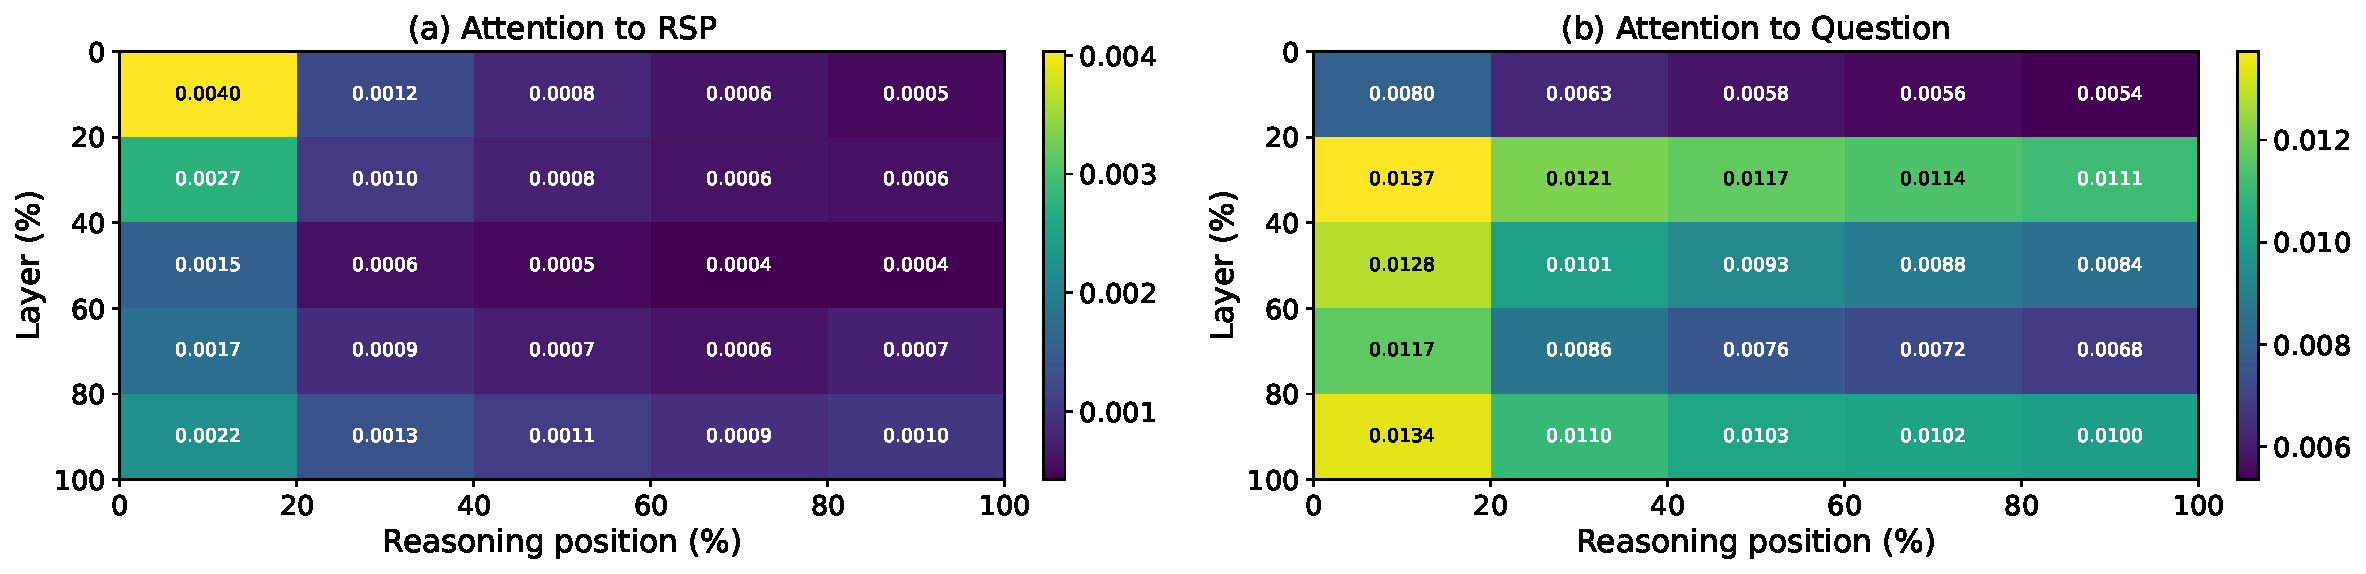
\includegraphics[width=0.72\textwidth]{img/attention/heatmap_qwen7b_suffix.pdf}
  \caption{Per-token attention mass on Qwen2.5-Math-7B (suffix, 500 MATH-500 problems, each with an independently sampled RSP). (a) RSP-token attention decreases along the reasoning-position axis (horizontal), consistent with the two-sided envelope of Eq.~\eqref{eq:sandwich}. The additional decrease along the layer axis (vertical) is a separate empirical observation suggesting that deeper layers sharpen the real-vs-random logit gap; it does not follow from Theorem~\ref{thm:decay} alone. (b) Question-token attention remains comparatively uniform. The reported quantity is the per-token mass of Appendix~\ref{app:attention_mass}, equal to $w_{r,i}^{(\ell)}/L$ averaged over heads and samples.}
  \label{fig:attention_mass}
\end{figure}

% ================================================================
\subsection{Branch opening and Pass@$N$ accumulation}\label{sec:multipath}
% ================================================================

The two envelopes outline the range within which RSP can influence a single rollout. We now ask how that influence appears in the output distribution and how it accumulates across rollouts.

We first justify the distribution choice. Theorem~\ref{thm:decay} and Proposition~\ref{prop:lower_env} use only attention identities and logit gaps---neither relies on isotropy. Branch opening, however, requires two distributional properties: an \emph{isotropic covariance} that distributes the variance budget uniformly over directions, and \emph{full support} that places positive probability on every nonempty open subset of the surrogate. The next theorem formalizes the first property at the per-RSP-token level---i.e., for the distribution of a single $\bar h\in\mathbb{R}^d$.

\begin{theorem}[Direction-agnostic minimax coverage]\label{thm:minimax_directional_coverage}
Let $D$ be any zero-mean distribution on $\mathbb{R}^d$ with covariance $\Sigma_D$ and trace budget $\mathrm{tr}(\Sigma_D)\le\rho^2$. Then $\min_{\|b\|=1}\mathrm{Var}_{h\sim D}(b^\top h) = \lambda_{\min}(\Sigma_D) \le \rho^2/d$, with equality if and only if $\Sigma_D = (\rho^2/d)\mathbf{I}_d$.
\end{theorem}

The proof is in Appendix~\ref{app:proofs}. Equality holds for \emph{any} distribution with isotropic covariance---Gaussianity is not the unique answer. Fixed prompts ($\Sigma_D=0$), PCA-aligned noise, vocabulary-token sampling, and embedding-covariance matching are all anisotropic and therefore strictly suboptimal in at least one direction. The reason to pick the Gaussian is the second property: an isotropic Gaussian has positive density everywhere on $\mathbb{R}^d$, so it commits to no particular direction (Lemma~\ref{lem:semantic_neutrality}). The two properties together enable the branch-opening guarantee below.

We now formalize branch opening on the surrogate. Linearizing the logits around $\bar h = 0$, define the affine surrogate $z_i^{\mathrm{lin}}(\bar h) := z_i + a_i^\top\bar h$ with $a_i := \nabla_{\bar h}z_i(0)$. For a baseline-excluded token $i$, the top-$K$ entry region is
\[
\mathcal{G}_{i,K} \;:=\; \bigl\{\bar h \in \mathbb{R}^d : \#\{j\neq i : z_j^{\mathrm{lin}}(\bar h) > z_i^{\mathrm{lin}}(\bar h)\} \le K-1\bigr\}.
\]
This matches the actual top-$K$ membership condition.

\begin{proposition}[Conditional top-$K$ entry]\label{prop:support_expansion}
Suppose $\mathcal{G}_{i,K}$ contains a nonempty open set. Since the isotropic Gaussian's full support assigns positive probability to it, $\mu_i := \Pr_{\bar h}(\bar h \in \mathcal{G}_{i,K}) > 0$.
\end{proposition}

The proof is in Appendix~\ref{app:proofs}. The mechanism guarantees that \emph{branches open} ($\mu_i > 0$); whether such a region exists is a task-side condition on the surrogate that is not automatically guaranteed. To lift this single-draw probability to task accuracy, we add two task-side assumptions: (M1) each independent RSP run produces a trajectory in the correct trajectory set with marginal probability at least $p_{\min}(x) > 0$, and (M2) the $N$ runs are mutually independent.

\begin{proposition}[Multi-path Pass@$N$]\label{prop:multi_path}
Under (M1)--(M2), with $N$ independent RSP runs,
\[
\Pr\!\big(\mathrm{Pass@}N\text{ on }x\big) \;\ge\; 1-(1-p_{\min}(x))^N \;\ge\; 1-\exp(-N\,p_{\min}(x)).
\]
\end{proposition}

The proof is in Appendix~\ref{app:proofs}. (M1) is task-side and not derivable from the mechanism alone---the mechanism is responsible only for \emph{admitting} baseline-excluded tokens into the candidate set, while whether an admitted branch is \emph{productive} depends on the task. Sharing one RSP across all samples eliminates this accumulation, so \emph{independence} is essential. The empirical signature of (M1) is reported in \S\ref{sec:experimental_analysis}.
